\section{Experiments}
\label{sec:experiments}

\subsection{Experimental Setup}

We evaluate Deep Attention Stimulation (DAS) on Qwen2.5-7B-Instruct,
an instruction-tuned large language model,
quantized to 4-bit precision using GPTQ~\citep{frantar2022gptq}.
All experiments use greedy decoding with fixed generation parameters,
including maximum generation length and decoding strategy,
to control for decoding variability and isolate the effect
of attention-level intervention.
This evaluation protocol follows prior analyses of quantized language models
that emphasize controlled decoding for mechanistic comparison
\citep{dettmers2022llmint8,lin2023awq}.

Evaluation prompts are drawn from IFEval~\citep{zhou2023ifeval},
a benchmark designed to test fine-grained instruction-following constraints
such as output language, formatting, casing, and structural requirements.
From the full benchmark, we identify failure cases in which
the full-precision model satisfies all verifiable constraints,
while the GPTQ-4bit model violates at least one.
We select ten representative samples for detailed evaluation,
covering diverse failure modes including unintended language switching,
formatting violations, constraint omission,
and degenerative repetition.

Crucially, this setup enables a controlled comparison between
instruction-following behavior before repair,
as exhibited by the quantized baseline,
and after attention-based repair,
under identical model weights and decoding conditions.

\subsection{Baseline and Intervention Settings}

We evaluate DAS under three stimulation strengths,
$\alpha \in \{0.0, 5.0, 10.0\}$.
When $\alpha = 0.0$, no corrective signal is injected,
and the model corresponds exactly to the unmodified GPTQ-4bit baseline.
We treat this setting as the before-repair condition.
The setting $\alpha = 5.0$ represents moderate stimulation,
intended to compensate attention heads most affected by quantization.
The setting $\alpha = 10.0$ represents excessive stimulation
and is used to examine the effect of over-intervention.

All before and after comparisons use the same quantized model
and identical decoding parameters,
with the only difference being the presence or absence
of attention-based stimulation.
This design ensures that observed differences
can be attributed to the intervention rather than confounding factors.

\subsection{Manual Evaluation Protocol}

Instruction-following failures often involve subtle qualitative violations
that are not reliably captured by automatic metrics 
\cite{lin2022truthfulqa, li2023evaluating}.
For this reason, all evaluations are conducted by manual inspection.
For each prompt, we derive a checklist of verifiable constraints
from the IFEval instruction,
including output language, casing, formatting,
punctuation, and structural requirements.

An output is labeled as recovered
if all constraints are satisfied,
partially recovered if at least one previously violated constraint
is corrected while others remain violated,
and failed otherwise.
Although IFEval provides automatic constraint-level scores,
prior work has shown that automatic metrics
can overlook instruction-level errors and qualitative failure modes
in large language model outputs
\citep{lin2022truthfulqa,li2023evaluating}.
Manual evaluation therefore remains necessary
for accurately assessing instruction adherence in complex prompts.

This protocol supports both controlled quantitative comparison
across samples and detailed qualitative case analysis.

\subsection{Qualitative Before and After Repair Case Studies}

\begin{figure*}[t]
  \centering
  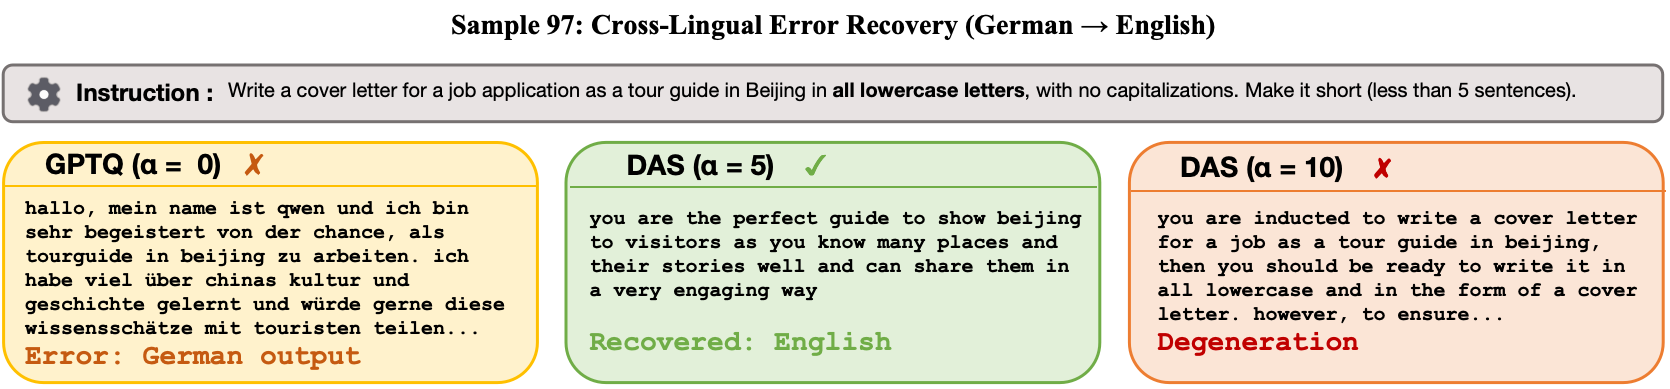
\includegraphics[width=\textwidth]{figures/figure3.png}
  \caption{Representative qualitative example illustrating instruction-following
  behavior before and after repair.
  Under GPTQ-4bit quantization with $\alpha = 0.0$,
  the model violates the instruction by producing German output.
  With moderate stimulation at $\alpha = 5.0$,
  the model recovers correct English output.
  Excessive stimulation at $\alpha = 10.0$
  destabilizes generation and leads to degenerative repetition.}
  \label{fig:qualitative}
\end{figure*}

We first examine representative qualitative cases
to illustrate how DAS alters instruction-following behavior.
Figure~\ref{fig:qualitative} presents a canonical cross-lingual failure case.
Before repair, the quantized model violates the language constraint,
despite satisfying the instruction under full precision.
After moderate stimulation,
the same model satisfies all instruction constraints.
In contrast, excessive stimulation destabilizes generation,
indicating that DAS functions as a repair mechanism
rather than a general performance enhancer.

% \begin{table*}[b!]
% \centering
% \small
% \begin{tabular}{@{}c>{\raggedright}p{3.5cm}p{3.8cm}p{3.8cm}p{3.8cm}@{}}
% \toprule
% \textbf{ID} & \textbf{Instruction Constraint} & \textbf{GPTQ ($\alpha=0$)} & \textbf{DAS ($\alpha=5$)} & \textbf{DAS ($\alpha=10$)} \\
% \midrule
% 57  & Zen-like style + lowercase + 3 bullets & \xmark{} Historical narrative style  & \cmark{} Abstract Zen metaphors      & \xmark{} Unstable symbols \\[0.3em]
% \textbf{97}  & \textbf{English lowercase letter}   & \xmark{} \textbf{German output (scored 1.0!)} & \cmark{} \textbf{Correct English}   & \xmark{} Repetitive text \\[0.3em]
% 74  & Limerick (AABBA) with highlights    & \xmark{} Broken rhyme scheme         & \xmark{} Still broken rhyme          & \xmark{} Collapsed output \\[0.3em]
% 79  & Letter frequency + no forbidden words & \cmark{} All constraints satisfied  & \cmark{} Maintained success          & \xmark{} Off-task meta-text \\[0.3em]
% 206 & 1930s jazz style + keyword ``rate''   & \cmark{} Proper song structure       & \xmark{} Severe repetition loop      & \xmark{} Continued repetition \\
% \bottomrule
% \end{tabular}
% \caption{Representative instruction-following behaviors under different stimulation strengths.
% \textbf{Sample 97} demonstrates cross-lingual recovery (German $\rightarrow$ English) 
% despite automatic metrics assigning perfect score (1.0) to the German output.
% \textbf{Sample 57} shows stylistic constraint recovery.
% \textbf{Sample 206} illustrates that DAS can degrade initially correct outputs.
% \textbf{Sample 74} remains unrecovered across all settings.
% \cmark{} indicates constraint satisfaction; \xmark{} indicates violation.
% Overall: 2/7 baseline failures recovered (28.6\%), 1/3 baseline passes degraded.}
% \label{tab:qualitative}
% \end{table*}

\begin{table*}[b!] 
\centering
\small
\begin{tabularx}{\textwidth}{@{} c >{\raggedright\arraybackslash}X >{\raggedright\arraybackslash}X >{\raggedright\arraybackslash}X >{\raggedright\arraybackslash}X @{}}
\toprule
\textbf{ID} & \textbf{Instruction Constraint} & \textbf{GPTQ ($\alpha=0$)} & \textbf{DAS ($\alpha=5$)} & \textbf{DAS ($\alpha=10$)} \\
\midrule
57  & Zen-like style + lowercase + 3 bullets & \xmark{} Historical narrative style  & \cmark{} Abstract Zen metaphors       & \xmark{} Unstable symbols \\[0.3em]
\textbf{97}  & \textbf{English lowercase letter}   & \xmark{} \textbf{German output (scored 1.0!)} & \cmark{} \textbf{Correct English}    & \xmark{} \textbf{Repetitive text} \\[0.3em]
74  & Limerick (AABBA) with highlights    & \xmark{} Broken rhyme scheme          & \xmark{} Still broken rhyme           & \xmark{} Collapsed output \\[0.3em]
79  & Letter frequency + no forbidden words & \cmark{} All constraints satisfied  & \cmark{} Maintained success           & \xmark{} Off-task meta-text \\[0.3em]
206 & 1930s jazz style + keyword ``rate''   & \cmark{} Proper song structure       & \xmark{} Severe repetition loop       & \xmark{} Continued repetition \\
\bottomrule
\end{tabularx}
\caption{Representative instruction-following behaviors under different stimulation strengths.
\textbf{Sample 97 is highlighted} because automatic metrics assigned a perfect score (1.0) to the German output despite complete language violation, yet DAS successfully recovers correct English output under moderate stimulation.
Sample 57 shows stylistic constraint recovery.
Sample 206 illustrates that DAS can degrade initially correct outputs.
Sample 74 remains unrecovered across all settings.
\cmark{} indicates constraint satisfaction; \xmark{} indicates violation.
Overall: 2/7 baseline failures recovered (28.6\%), 1/3 baseline passes degraded.}
\label{tab:qualitative}
\end{table*}

Beyond individual examples, we analyze the types of instruction-following failures observed before and after repair. Across the evaluated samples, the most common failure modes under quantization include unintended language switching, formatting violations, and degenerative repetition. Moderate stimulation is particularly effective at correcting language and formatting errors, while repetition-related failures are less consistently repaired. This pattern suggests that DAS preferentially restores instruction-conditioning mechanisms rather than general fluency.

Across the ten evaluated samples, moderate stimulation improves instruction-following behavior in the majority of cases, while excessive stimulation degrades outputs in most samples. Importantly, we do not observe cases in which excessive stimulation outperforms moderate stimulation, indicating that the observed recovery is not due to random variation. Taken together, these results establish a consistent before-and-after contrast in instruction-following behavior (see Table~\ref{tab:qualitative} for representative cases). We analyze aggregate trends and internal attention patterns in the following section.
